\documentclass[a4paper, 12pt]{scrreprt}
\usepackage[german]{babel}
\usepackage[german]{translator}
\usepackage[utf8]{inputenc}
\usepackage[T1]{fontenc}
\usepackage{ae}
\usepackage[bookmarks,bookmarksnumbered]{hyperref}
\usepackage{graphicx}
\usepackage{color}
\usepackage[dvipsnames]{xcolor}
\usepackage{booktabs}
\usepackage{longtable}
\usepackage{listings}
\usepackage{tabularx}
\usepackage[left=2.50cm, right=2.50cm, bottom =3.53cm]{geometry}
\usepackage{ pdflscape}
%\usepackage{pdfpages}
%\usepackage[section]{placeins}


\newcommand{\col}[2]{\textcolor{#1}{#2}}

% Zeilenhöhe bei Tabellen
\newcommand{\zh}[1]{\parbox[0pt][#1][c]{0cm}{}}

\begin{document}
	\thispagestyle{plain}
	
	\begin{titlepage}
		\begin{center}
			\begin{figure}[ht]
				\centering
				
\includegraphics[width=0.66\textwidth, angle=0]{logo/name_blau_ofCourse.jpg}
			\end{figure}
			
			\begin{title}
				\title{\Huge{\textbf{Kurseinheiten-Manager \\ \ \\ 
							\ \\
							Handbuch Installation
							}}}
			\begin{figure}[th]
				\centering
				
\includegraphics[width=0.40\textwidth, angle=0]{Grafiken/installation-instructions-icon}
			\end{figure}
				
			\end{title}
			\hspace{3cm}
			
			Software Engineering Praktikum \\
			Sommersemester 2015\\
			Universität Passau\\
			
			
			Betreuer: Andreas Stahlbauer \\
        	\hspace{1,5cm}\\
        	Version: 1.1 \\
        	\hspace{1,5cm}\\
        	Datum: 10.7.2015\\[28pt]
        	Team 3 \\

			\ \\
        \begin{tabular}{ | l | l | l | l |}
        	\hline
        	\textbf{Matrikelnummer} & \textbf{Name} & \textbf{Phase} & \textbf{E-Mail}  \\ \hline
        	63097 & Katharina Hölzl & Pflichtenheft & hoelzlka@fim.uni-passau.de \\ \hline
        	64504 & Ricky Strohmeier& Entwurf & strohric@fim.uni-passau.de  \\ \hline
        	61085 & Sebastian Schwarz & Feinspezifikation & sebastian@nrschwarz.de \\ \hline 
        	64080 & Tobias Fuchs & Implementierung  &  fuchstob@fim.uni-passau.de\\ \hline
        	58379 & Patrick Cretu  &  Validierung & cretu@fim.uni-passau.de \\ \hline
        \end{tabular}
        
      
       
        
        
    \end{center}
\end{titlepage}


% Platzierung des Inhaltsverzeichnisses
\tableofcontents
\chapter{Benötigte Software}
Für die Vorbereitung, Einrichtung und Inbetriebnahme der Webapplikation \textbf{ofCourse} wird folgende Software benötigt.
\begin{itemize}
	\item Java Runtime Environment 8\\
	{\it Link:\\} \url{https://www.java.com/de/download/}
	\item Apache Tomcat 8\\
	{\it Link:\\} \url{https://tomcat.apache.org/download-80.cgi}
	\item 7-zip\\
	{\it Link:\\} \url{http://www.7-zip.de/}
	\item Notepad++ (oder einen Texteditor Ihrer Wahl)\\
	{\it Link:\\} \url{https://notepad-plus-plus.org/download/v6.7.9.2.html}
	\item Webbrowser(z.B. Firefox 38)\\
	{\it Link:\\} \url{https://www.mozilla.org/de/firefox/new/}
	\item PostgreSQL Datenbank\\
	{\it Link:\\} \url{http://de.enterprisedb.com/products-services-training/pgdownload}
\end{itemize}
\chapter{Einrichtung des Tomcat Servers}
\section{Windows}
\paragraph{The simple way}\ \\
\ \\
Laden Sie die JRE von URL
\begin{center}
	 \url{https://www.java.com/de/download/}
\end{center}
und installieren Sie es auf ihrem System.\ \\
\ \\
Laden Sie nun den Tomcat Windows Installer von URL 
\begin{center}
	\url{https://tomcat.apache.org/download-80.cgi}
\end{center}
herunter und starten Sie den Installationsvorgang indem Sie die heruntergeladene Datei doppelklicken.\\
Fuehren Sie das Setup durch, bis Sie auf die Seite {\it Configuration} kommen.
\begin{figure}[h]
\centering
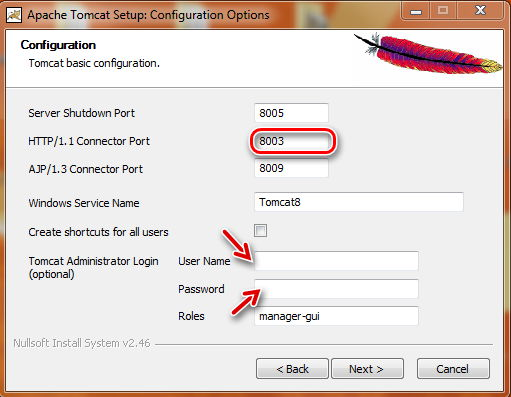
\includegraphics[width=0.75\linewidth]{Grafiken/TomcatInstall1}
\caption{Seite Configuration des Tomcat Setups}
\label{fig:TomcatInstall1}
\end{figure}\\
Aendern Sie den {\it HTTP/1.1 Connector Port} auf \textbf{8003} und legen Sie einen {\it User Name} und ein {\it Password} fuer den Administrator fest.(vgl Abbildung \ref{fig:TomcatInstall1})\\
\newpage
\ \\
Auf der darauffolgenden Seite des Setups werden Sie aufgefordert den Pfad der {\it Java Virtual Machine} anzugeben.\\
Geben Sie hier den Pfad der im vorherigen installierten {\it Java Runtime Environment} an.\\
\ \\
Fuehren Sie nun die Installation zu Ende indem Sie das restliche Setup durchlaufen.\\
Ihr Tomcat Server ist nun installiert.
\ \\
Wechseln Sie nun in da Installationsverzeichnis des Tomcat Servers. Dort finden Sie folgende Dateien:
\begin{figure}[h]
\centering
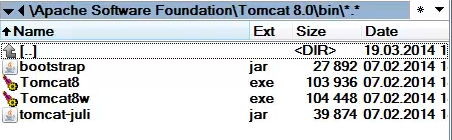
\includegraphics[width=0.8\linewidth]{Grafiken/TomcatDirectory}
\caption{Installationsverzeichnis}
\label{fig:TomcatDirectory}
\end{figure}\\
\newpage
\ \\
Durch Klicken auf die Datei {\it Tomcat8} starten Sie den Tomcat Server direkt.\\
\ \\
Durch Klicken auf die Datei {\it Tomcat8w} oeffnen Sie ein Fenster in dem Sie den Server weiter konfigurieren koennen und durch 
Betaetigen des \textbf{Start} Buttons starten Sie den Server.
\begin{figure}[h]
\centering
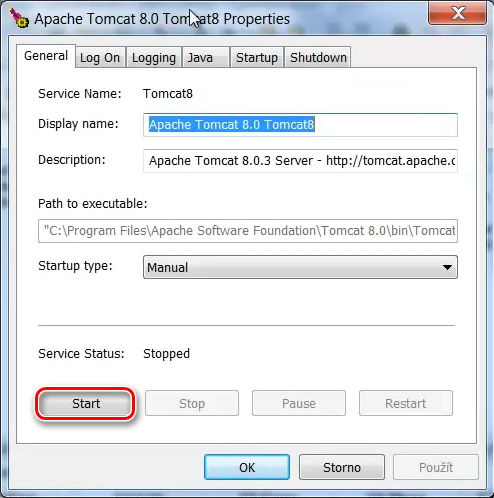
\includegraphics[width=0.8\linewidth]{Grafiken/TomcatStartup}
\caption{Start/Konfigurationsfenster des Tomcat Servers}
\label{fig:TomcatStartup}
\end{figure}

\newpage
\ \\
\ \\
\ \\
\ \\
\paragraph{The long and hard way}\ \\
\ \\
Wenn Sie nicht den Installer verwenden wollen, folgen Sie bitte den Anweisungen unter:
\begin{center}
	\url{http://tomcat.apache.org/tomcat-8.0-doc/RUNNING.txt}
\end{center}
\newpage
\section{Linux}
\subsection{Installation von Java Development Kit 8}
Die aktuelle Version des {\it Java Development Kit 8} finden Sie unter
\begin{center}
	\url{http://www.oracle.com/technetwork/java/javase/downloads/jdk8-downloads-2133151.html}
\end{center}
Laden Sie sich hier das JDK für ihr System herunter.\\
Öffnen Sie ein Terminal in ihrem Linux - System und wechseln Sie in den Ordner, in dem Sie das heruntergeladene JDK gespeichert haben.\\
\ \\
Entpacken Sie das heruntergeladene JDK mit dem Befehl
\begin{center}
	tar -zxvf {\it \{JDK - Datei mit der Endung .tar.gz\} }
\end{center}
Beispielsweise:
\begin{center}
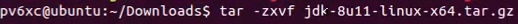
\includegraphics[width=0.85\linewidth]{Grafiken/Linux_Java_pfad}
\end{center}
Wechseln Sie nun in den Ordner {\it usr$/$lib} und erzeugen Sie dort einen {\it java} - Ordner mit dem Befehl
\begin{center}

\includegraphics[width=0.6\linewidth]{Grafiken/Linux_create_java}
\end{center}
Verschieben Sie nun den extrahierten JDK - Ordner in das eben erstellte java - Verzeichnis.\\
Wechseln Sie dafür in den Ordner in dem das JDK liegt und verschieben Sie den Ordner mittels des Befehls
\begin{center}
	sudo mv \{{\it JDK - Ordner}\} $/$usr$/$lib$/$java
\end{center}
Beispielsweise: 
\begin{center}
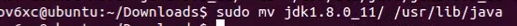
\includegraphics[width=0.75\linewidth]{Grafiken/Linux_Move_befehl}
\end{center}
Wechseln Sie nun in den JDK - Ordner. \\
Führen Sie nun folgende Befehle nacheinander im Terminal aus. Ersetzen Sie dabei die JDK - Version durch die Version ihres heruntergeladenen JDK.
\begin{center}
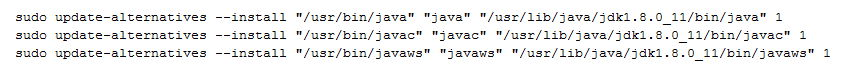
\includegraphics[width=1.1\linewidth]{Grafiken/Liunux_befehle}
\end{center}
\newpage
\ \\
Nun müssen Sie noch den \textbf{JAVA\_HOME} Pfad in ihrer {\it ~/.bashrc} - Datei setzen.\\
Öffnen Sie diese und fügen Sie am Ende folgendes ein(mit angepasster JDK - Versionsnummer):
\begin{center}
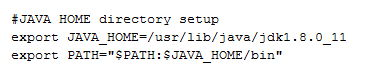
\includegraphics[width=0.7\linewidth]{Grafiken/JAVAHome}
\end{center}

\subsection{Installation von Tomcat 8}
Laden Sie sich unter 
\begin{center}
	\url{http://tomcat.apache.org/download-80.cgi}
\end{center}
unter dem Abschnitt {\it Binary Distributions} die aktuellste Version des Tomcat - Servers im .zip - Format herunter.\\
Öffnen Sie ein Terminal in ihrem Linux - System und wechseln Sie in den Ordner, in den Sie dem heruntergeladenen Tomcat -Server gespeichert haben.\\
\ \\
Entpacken Sie den heruntergeladenen Tomcat mit dem Befehl
\begin{center}
	unzip  {\it \{Apache Tomcat - Datei mit der Endung .zip\} }
\end{center}
In dem Ordner befindet sich nun der entpackte Tomcat - Ordner.\\
\ \\
Wechseln Sie nun in den Ordner {\it $/$usr} und erzeugen Sie dort einen {\it apache} - Ordner mit dem Befehl
\begin{center}

\includegraphics[width=0.5\linewidth]{Grafiken/apache_linux_path}
\end{center}
\ \\
Verschieben Sie nun den extrahierten Tomcat - Ordner in das eben erstellte apache - Verzeichnis.\\
Wechseln Sie dafür in den Ordner in dem der Tomcat Server liegt und verschieben Sie den Ordner mittels dem Befehl
\begin{center}
	sudo mv \{{\it Apache Tomcat - Ordner}\} $/$usr$/$apache
\end{center}
Wechseln Sie nun in dem Tomcat Server - Ordner mit dem Befehl({\it Versionsnummer an heruntergeladenen Server anpassen})
\begin{center}
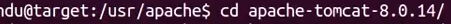
\includegraphics[width=0.65\linewidth]{Grafiken/wechseln_server_ordner}
\end{center}
Geben Sie nun folgenden Befehl ein({\it Versionsnummer an heruntergeladenen Server anpassen}):
\begin{center}
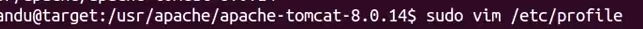
\includegraphics[width=0.9\linewidth]{Grafiken/Befhel}
\end{center}
\newpage
\ \\
Es öffnet sich nun eine Datei. Fügen Sie in diese Datei die im folgenden abgebildeten Zeilen ein ({\it Versionsnummer an heruntergeladenen Server anpassen}).
\begin{figure}[h]
\centering
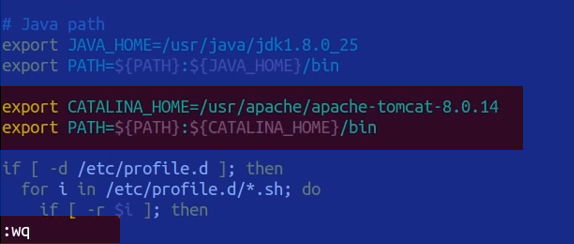
\includegraphics[width=0.7\linewidth]{Grafiken/Catalina_Home}
\caption{Definieren des CATALINA - Homeverzeichnises}
\label{fig:Catalina_Home}
\end{figure}
\ \\
Führen Sie nun anschließend noch folgenden Befehl aus:
\begin{center}
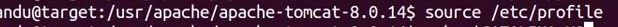
\includegraphics[width=0.8\linewidth]{Grafiken/Befehl_idonKnow}
\end{center}
\ \\
Wechseln Sie jetzt in das {\it$/$bin} des Tomcat Servers
\begin{center}

\includegraphics[width=0.7\linewidth]{Grafiken/Bin_direct}
\end{center}
\ \\
Dort müssen Sie nun noch die Zugriff- bzw. Ausführungsrechte der Dateien ändern, damit Sie nachher den Server auch starten und beenden können. Die Rechte ändern Sie durch Eingabe des folgenden Befehls:
\begin{center}
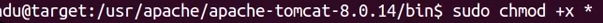
\includegraphics[width=0.8\linewidth]{Grafiken/rechte}
\end{center}
\ \\
Da Sie nun die entsprechenden Berechtigungen besitzen, können Sie den Server mit folgendem Befehl starten:
\begin{center}

\includegraphics[width=0.8\linewidth]{Grafiken/Tomcat_starten_linux}
\end{center}
\ \\
Öffnen Sie nun ihren Browser und geben folgende URL ein
\begin{center}
	{\it http://localhost:8080}
\end{center}
Sie sehen nun die Startseite des Tomcat Servers.\begin{figure}
\centering
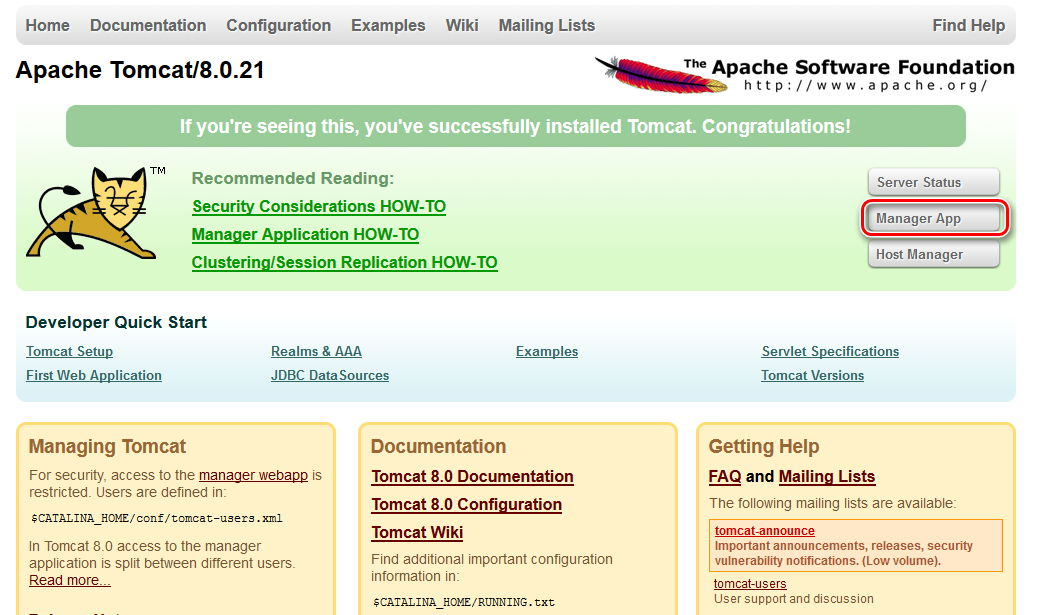
\includegraphics[width=0.8\linewidth]{Grafiken/ServerStartPage}
\caption{Startseite des Tomcat Servers}
\label{fig:ServerStartPage1}
\end{figure}
\ \\
\newpage
\ \\
Bevor Sie nun  auf die Managementseite des Tomcat Servers gelangen können, auf der Sie wie in {\it Kapitel 4 beschrieben}, Web - Applikationen deployen können, müssen Sie einen Benutzer autorisieren indem Sie einen Benutzernamen und ein Passwort festlegen.\ \\
\ \\
Wechseln Sie dafür wieder aus dem {\it$/$ bin} - Ordner des Tomcat Servers zurück in den Hauptordner des Servers.\\
Geben Sie dann folgenden Befehl ein:
\begin{center}
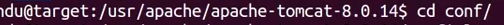
\includegraphics[width=0.7\linewidth]{Grafiken/conf-ordner}
\end{center}
\ \\
Damit wechseln Sie in den {\it $/$conf} - Ordner der Servers, welcher Konfigurationsdateien enthält.\\
Öffnen Sie nun die Datei {\it tomcat-users.xml}.\\
Diese öffnen Sie mit folgendem Befehl:
\begin{center}
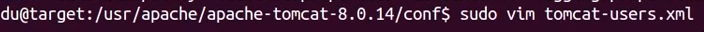
\includegraphics[width=0.8\linewidth]{Grafiken/zomcat_users}
\end{center}
\newpage
\ \\
In der geöffneten Datei tragen Sie nun folgende Informationen ein:
\begin{figure}[h]
\centering
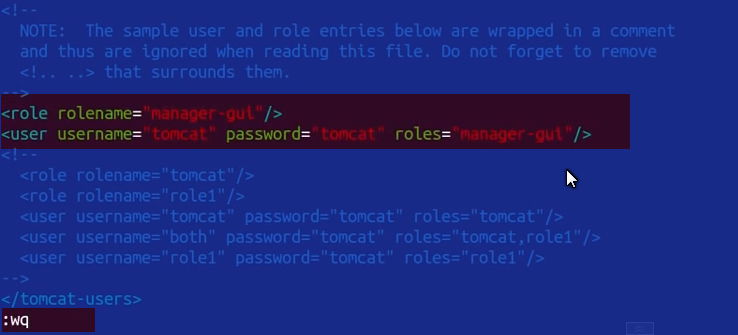
\includegraphics[width=0.7\linewidth]{Grafiken/server-user+}
\caption{Hinzufügen eines neuen Benutzers zum Tomcat Server}
\label{fig:server-user+}
\end{figure}
\ \\
Zusätzlich ändern wir nun noch den Port des Servers von 8080 auf 8003.\\
Dafür geben Sie folgenden Befehl in das Terminal ein
\begin{center}
	sudo vim server.xml
\end{center}
In der geöffneten Datei finden Sie den Abschnitt:
\begin{figure}[h]
\centering
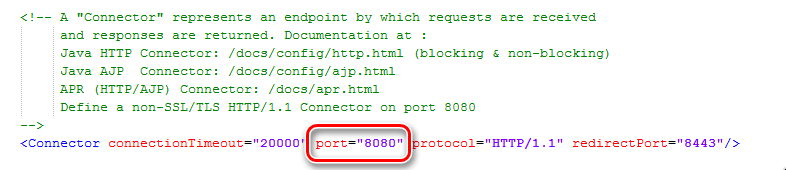
\includegraphics[width=0.9\linewidth]{Grafiken/port8080}
\caption{Server.xml vor Änderung}
\label{fig:port8080}
\end{figure}
\ \\
Ändern Sie den Port zu \textbf{8003}. Fügen Sie zusätzlich am Ende des Dokuments folgendes ein:
\begin{center}
	{\it :wq}
\end{center}
Nach Betätigen der Eingabetaste wird damit die geöffnete Datei gespeichert und geschlossen.\ \\
\ \\
Wechseln Sie nun wieder, wie bereits oben beschrieben, in den {\it $/$bin} - Ordner des Tomcat Servers.\\
\ \\
Hier beenden Sie nun den Server durch Eingabe des Befehls 
\begin{center}
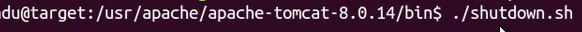
\includegraphics[width=0.8\linewidth]{Grafiken/Shutdown}
\end{center}
\ \\
Sie starten den Server erneut mit dem Befehl
\begin{center}
	
\includegraphics[width=0.8\linewidth]{Grafiken/Tomcat_starten_linux}
\end{center}
\ \\
Öffnen Sie nun ihren Browser und geben folgende URL ein
\begin{center}
	{\it http://localhost:8003}
\end{center}
\ \\
Sie sehen nun erneut die Startseite des Tomcat Servers.
\begin{figure}[h]
	\centering
	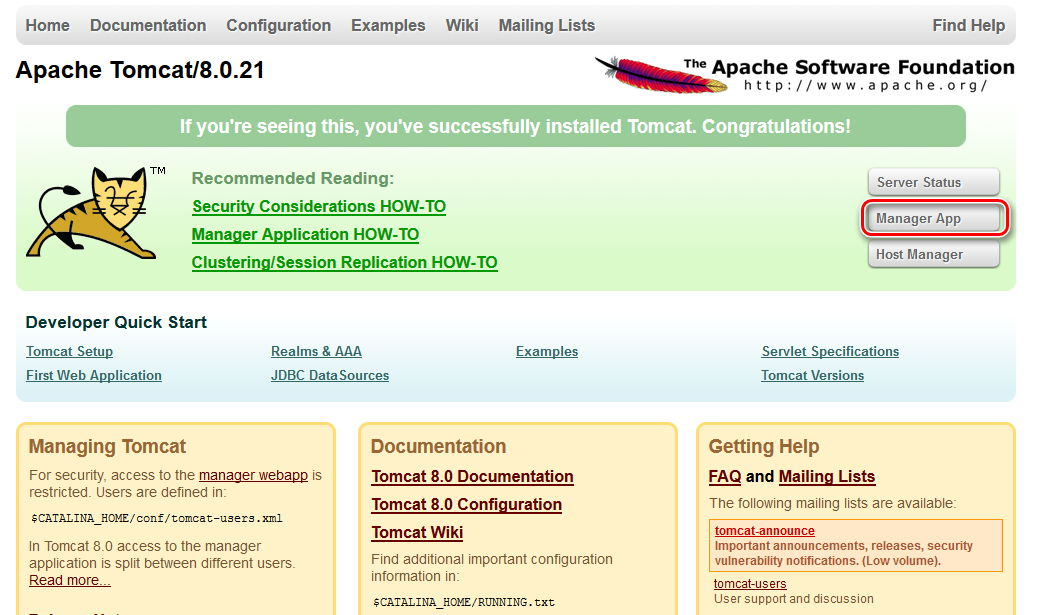
\includegraphics[width=0.8\linewidth]{Grafiken/ServerStartPage}
	\caption{Startseite des Tomcat Servers}
	\label{fig:ServerStartPage12}
\end{figure}
\ \\
Durch Betätigen des Buttons {\it Manager App} und Eingabe der vorhin\ref{fig:server-user+} festgelegten Zugangsdaten
\begin{center}
	{\it Benutzername:} tomcat \\
	{\it Passwort:} tomcat 
\end{center} werden Sie auf die Verwaltungsseite des Servers weitergeleitet, wo Sie u.a. Web - Applikationen deployen können({\it vgl. Kapitel 4}).

\chapter{Vorbereitung von ofCourse}
Öffnen Sie die Datei \textbf{ofCourse.war} mit der Software {\it 7Zip}.\\
Sie sehen nun die im folgenden abgebildeten Ordner:
\begin{figure}[h]
\centering
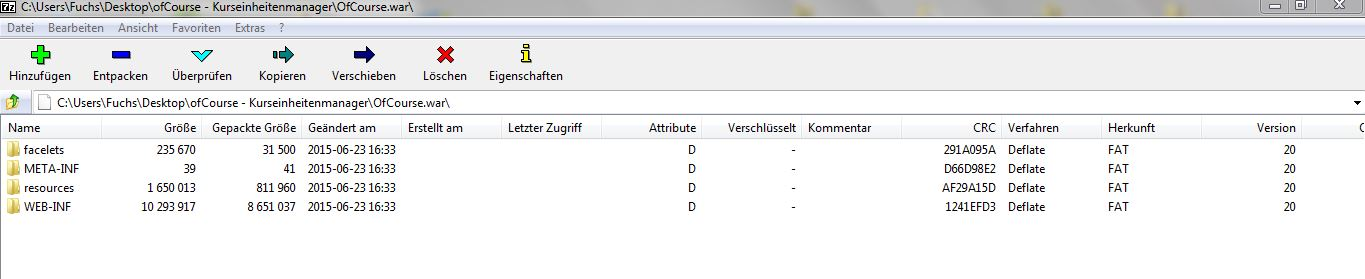
\includegraphics[width=1.0\linewidth]{Grafiken/7ZipOfCourse1}
\caption{ofCourse.war in 7Zip geoeffnet}
\label{fig:7ZipOfCourse1}
\end{figure}\\
Navigieren Sie nun zum Ordner \textbf{config}. Diesen erreichen Sie folgendermaßen:
\begin{center}
	{\it WEB-INF > config}
\end{center}
In diesem Ordner finden Sie die Dateien:
\begin{itemize}
	\item ofCourse.properties
	\item mail.properties
\end{itemize}
Diese öffnen Sie nun jeweils mit {\it Notepad++ (oder einem Texteditor Ihrer Wahl)}. Füllen diese Dateien mit ihren Daten und speichern Sie. 
\begin{figure}[h]
\centering
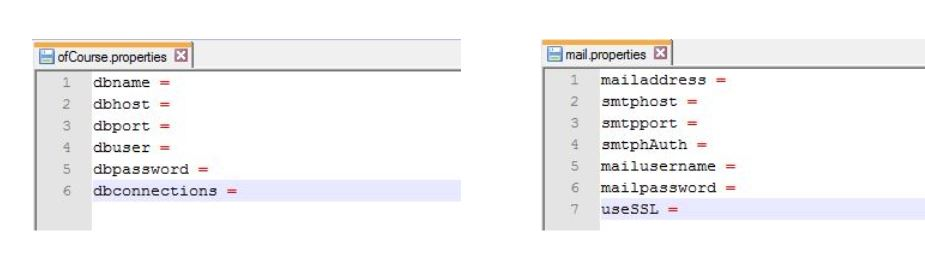
\includegraphics[width=0.7\linewidth]{Grafiken/propertiesComplete}
\caption{Zu füllende Dateien}
\label{fig:propertiesComplete}
\end{figure}\ \\
\textbf{ofCourse} ist nun mit ihren Daten konfiguriert.\\
\chapter{Deployment ofCourse}
Starten Sie nun ihren Tomcat Server. Durch Eingabe von
\begin{center}
		{\it http://localhost:8003}
\end{center}
werden Sie auf die Startseite des Servers geleitet. Hier Betätigen Sie den Button \textbf{Manager App} auf der rechten Seite.
\begin{figure}[h]
\centering
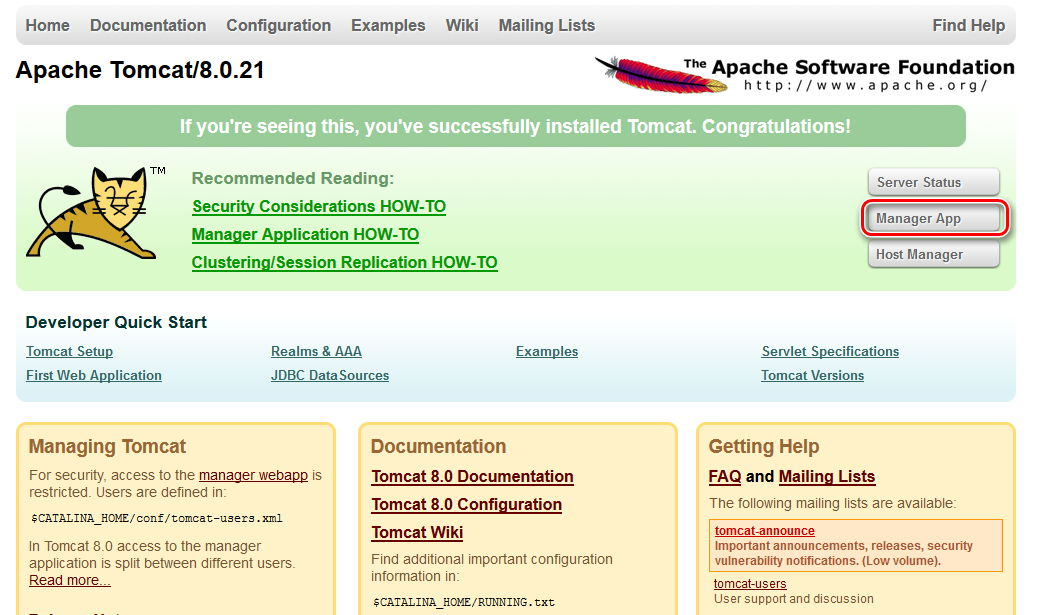
\includegraphics[width=0.8\linewidth]{Grafiken/ServerStartPage}
\caption{Startseite des Tomcat Servers}
\label{fig:ServerStartPage}
\end{figure}\\
Sie werden nun aufgefordert ihre Zugangsdaten einzugeben. Geben Sie die Daten ein, die Sie in {\it Kapitel 2 Einrichten des Tomcat Servers} gewählt haben. 
\newpage 
\ \\
Sie werden nun auf die \textbf{Tomcat Web Application Manager} Seite weitergeleitet.
Scrollen Sie nach unten, bis Sie den {\it Deploy} - des Servers sehen.
\begin{figure}[h]
\centering
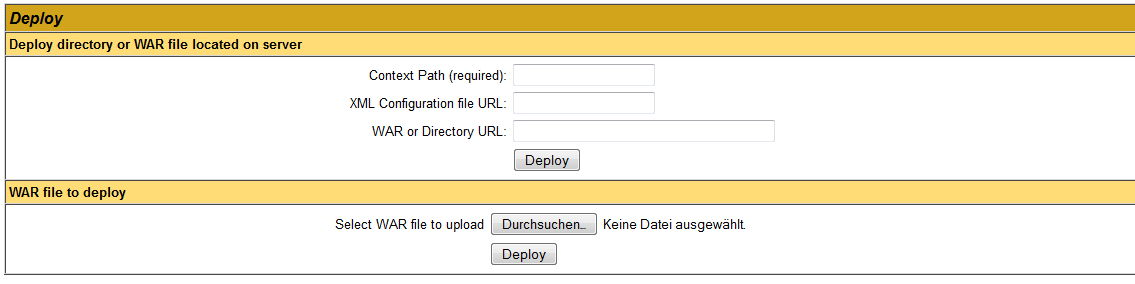
\includegraphics[width=0.9\linewidth]{Grafiken/ServerDeploy}
\caption{Deploybereich des Tomcat Servers}
\label{fig:ServerDeploy}
\end{figure}
\\
Druecken Sie nun im Abschnitt {\it WAR file to deploy} den \textbf{Durchsuchen} Button und waehlen sie die {\it ofCourse.war} - Datei aus. Durch Betätigen des Buttons \textbf{Deploy} wird die .war - Datei im Server depolyed.\\
\ \\
Sie sehen nun {\it ofCourse} im {\it Application} - Bereich des Servers.
\begin{figure}[h]
\centering
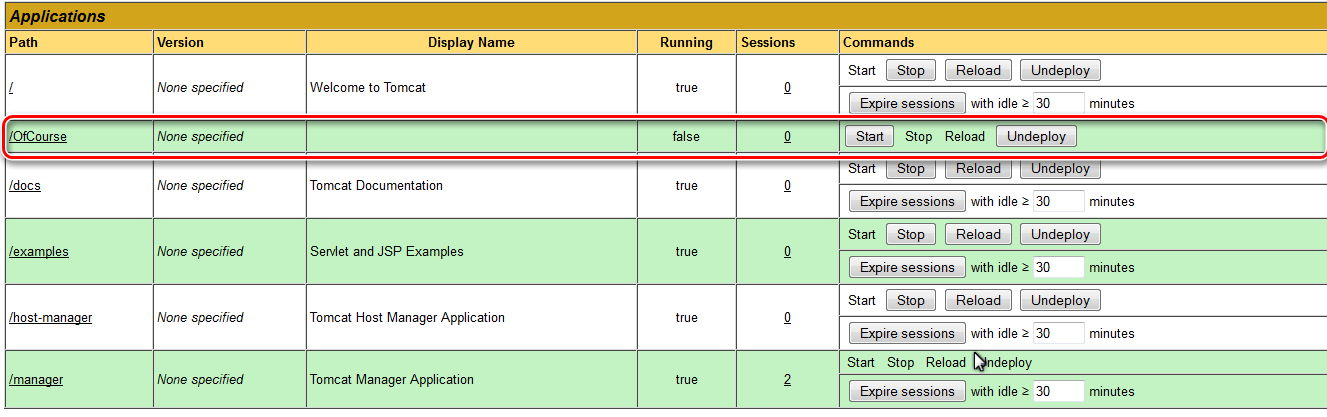
\includegraphics[width=0.9\linewidth]{Grafiken/ApplicationBereichServerDeployed}
\caption{Application Bereich des Tomcat Servers}
\label{fig:ApplicationBereichServerDeployed}
\end{figure}
\ \\
\textbf{ofCourse} laeuft nun noch nicht auf ihrem Server. Um die Applikation zu starten, druecken Sie den \textbf{Start} Button bei dem Eintrag {\it ofCourse}.
\begin{figure}[ht]
\centering
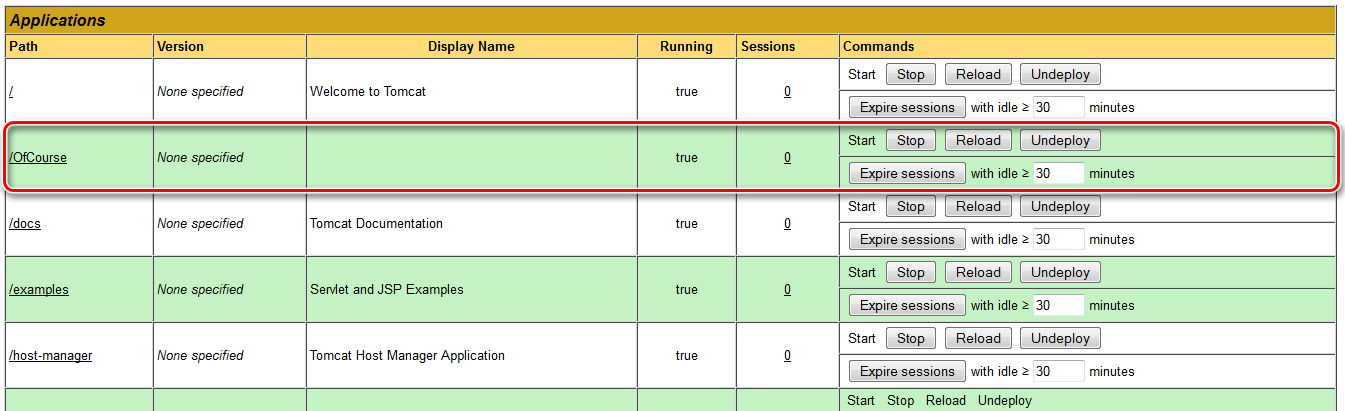
\includegraphics[width=0.9\linewidth]{Grafiken/ofCourseDeployed}
\caption{ofCourse laeuft auf dem Server}
\label{fig:OfCourseDeployed}
\end{figure}
\newpage
\ \\
\textbf{ofCourse} laeuft nun auf dem Server. Hier können sie auch einstellen nach wie vielen Minuten ohne Taetigkeit die Session zerstoert werden soll.\ \\
\ \\
Geben Sie nun im Browser 
\begin{center}
	{\it http://localhost:8003/OfCourse/}
\end{center}
Sie befinden sich nun auf der Startseite von \textbf{ofCourse}.
\begin{figure}[h]
	\centering
	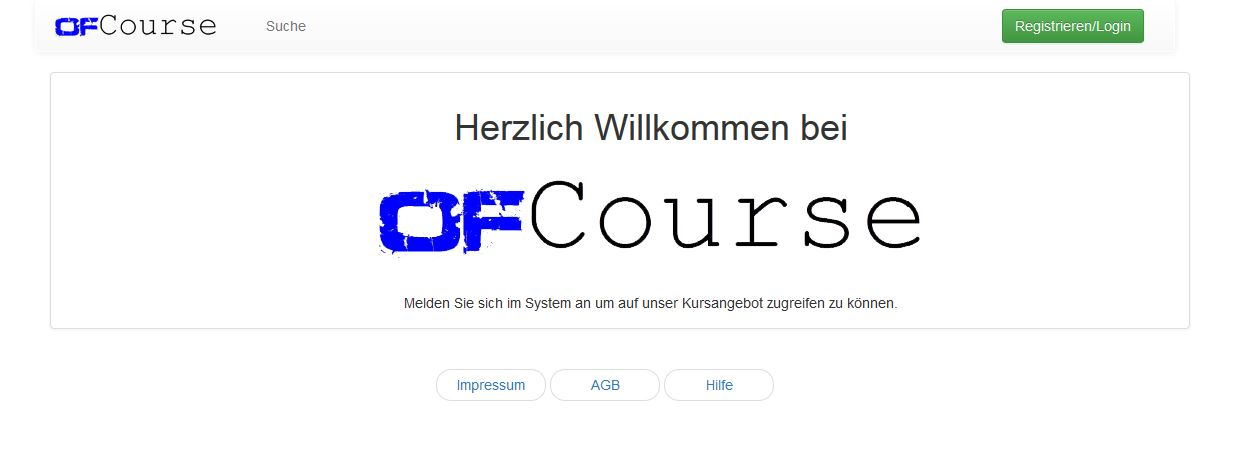
\includegraphics[width=0.8\linewidth]{Grafiken/indexPage}
	\caption[]{Startseite von ofCourse}
	\label{fig:indexPage1}
\end{figure} 

\chapter{Erster Login}
Geben Sie in ihren Browser folgende URL ein:
\begin{center}
	{\it http://localhost:8003/OfCourse/}
\end{center}
Sie befinden sich nun auf der Startseite von \textbf{ofCourse}.
\begin{figure}[h]
\centering
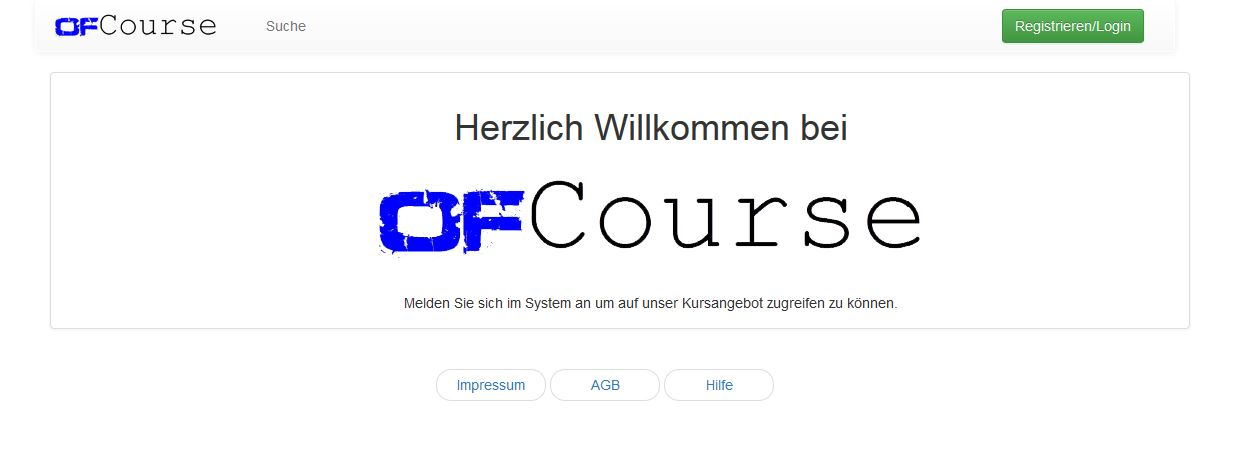
\includegraphics[width=0.8\linewidth]{Grafiken/indexPage}
\caption[]{Startseite von ofCourse}
\label{fig:indexPage}
\end{figure} \ \\
Durch Betätigen des  gruenen Buttons \textbf{Registrieren/Login} links oben auf der Startseite werden Sie auf die Anmeldeseite weitergeleitet.
\begin{figure}[h]
\centering
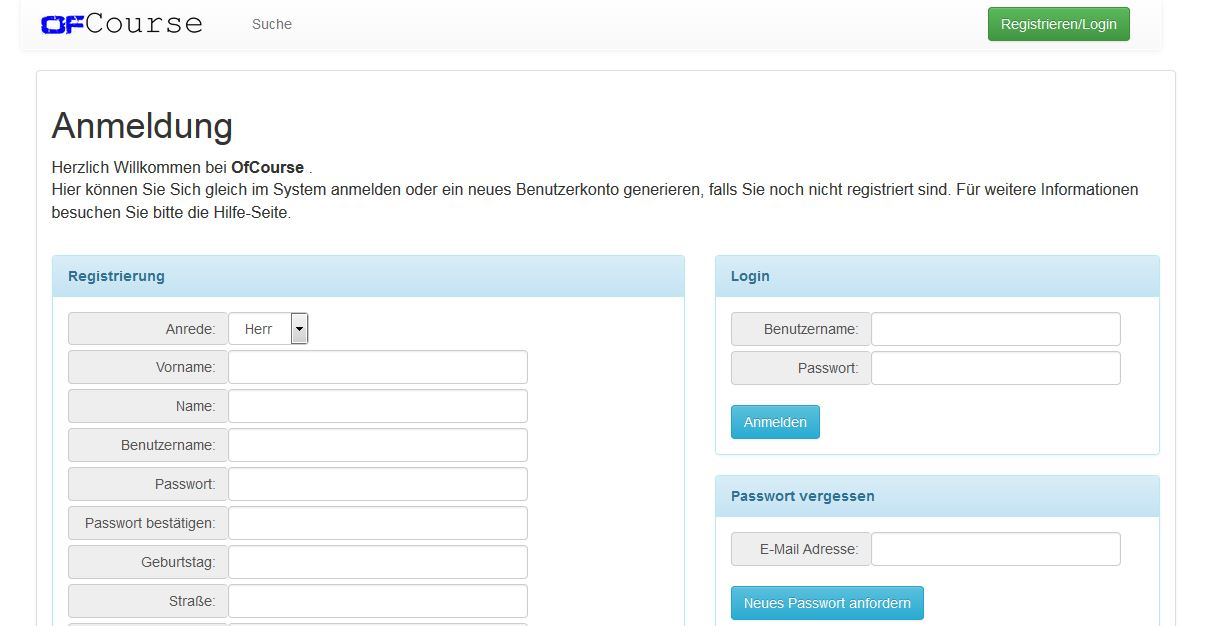
\includegraphics[width=0.8\linewidth]{Grafiken/loginPage}
\caption{Ausschnitt der Anmeldeseite}
\label{fig:loginPage}
\end{figure} \newpage
\ \\
Füllen Sie nun die Felder {\it Benutzername} und {\it Passwort} mit folgenden Daten aus und Betätigen Sie den \textbf{Anmelden} Button.
\begin{center}
	Benutzername: {\it admin1}\\
	Passwort: {\it Password!123}
\end{center}
Sie werden nun auf die \textbf{Meine Kurse} Seite weitergeleitet und sind nun erfolgreich im System angemeldet.
\begin{figure}[h]
\centering
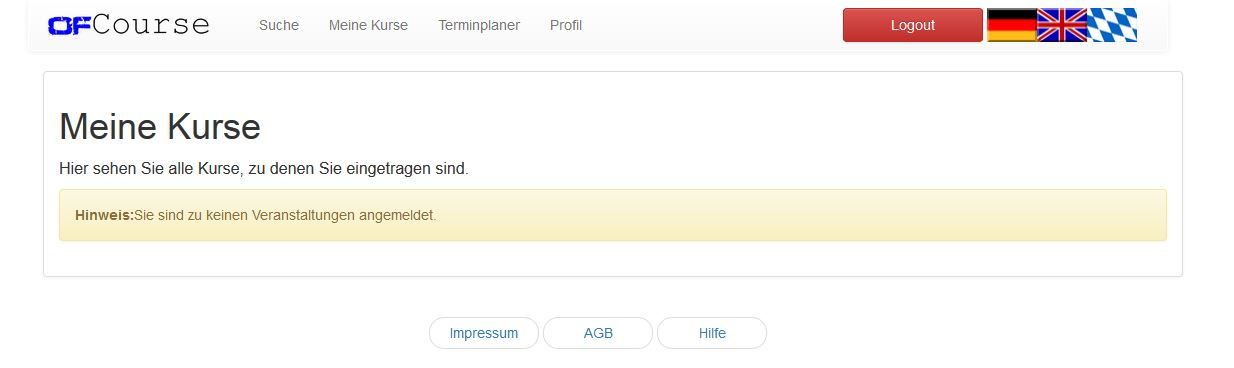
\includegraphics[width=0.8\linewidth]{Grafiken/myCoursesPage}
\caption{'Meine Kurse' - Seite von ofCourse}
\label{fig:myCoursesPage}
\end{figure}
\ \\
\ \\
\begin{center}
	{\Large Herzlich Willkommen bei \ \\}
	\ \\

\includegraphics[width=0.5\linewidth]{logo/name_blau_ofCourse}
\end{center}

\end{document}